
\section{Comunicación y supervisión}\label{sec:montaje_comunicaciones}

La arquitectura de comunicaciones se definió en el segundo corte y el software de la supervisión remota (la API, la base de datos y la interfaz) ya está desarrollado. En el tercer corte, la cadena completa se verificó con el prototipo (VAL-10). Esta sección presenta la arquitectura, el software desarrollado, el estado de cada parte y las verificaciones realizadas. La propuesta completa, elaborada por el integrante Juan Camilo Díaz Gamboa, se incluye en el Anexo~\ref{anx:arquitectura_com}.

\paragraph{Arquitectura propuesta.} La arquitectura separa la red de control local de la capa de supervisión remota (Figura~\ref{fig:arquitectura_iot}). En el nivel de control, el PLC Siemens S7-1200 CPU 1214C adquiere las señales de campo y acciona los actuadores, de modo que el ciclo de limpieza no depende de ningún equipo externo. El PLC, la HMI KTP600 Basic y la pasarela de supervisión se conectan en estrella a través del switch Siemens CSM 1277, que solo conmuta tramas (capa 2). La Raspberry Pi, con Node-RED, actúa como pasarela entre el PLC y los servicios externos: lee las variables del PLC y las envía a una API, desde donde las consume la interfaz de supervisión remota. Como la Raspberry Pi concentra la conexión con el exterior, el PLC no queda expuesto directamente a Internet \cite{hajda2021security}. En la propuesta, la Raspberry Pi se une a la misma red local por WiFi, mediante un punto de acceso o router conectado al switch en modo puente; la conexión de la Raspberry Pi con la red se verificó con la cadena completa (VAL-10). En la etapa final no se requiere un computador: este solo se usa para programar el PLC y la HMI.

\begin{figure}[H]
\centering
\begin{tikzpicture}[
  font=\footnotesize,
  nodo/.style={draw=AzulUSTA,rounded corners=3pt,fill=AzulUSTA!8,align=center,minimum height=1.1cm,text width=2.5cm},
  cond/.style={draw=AzulUSTA,dashed,rounded corners=3pt,fill=white,align=center,minimum height=1.1cm,text width=2.5cm},
  enlace/.style={line width=0.7pt,draw=AzulUSTA},
  etiqueta/.style={font=\scriptsize,align=center,fill=white,inner sep=1pt}]
  \node[nodo] (plc) at (0,2.6) {PLC S7-1200\\CPU 1214C};
  \node[nodo] (sw) at (0,0) {Switch\\CSM 1277};
  \node[nodo] (hmi) at (-4.2,0) {HMI\\KTP600 Basic};
  \node[cond] (ap) at (4.2,0) {Punto de acceso\\WiFi\\(condicional)};
  \node[nodo] (rpi) at (8.4,0) {Raspberry Pi\\(Node-RED)};
  \node[nodo] (api) at (8.4,-2.6) {API (FastAPI)\\y SQLite};
  \node[nodo] (web) at (4.2,-2.6) {Interfaz web\\(Streamlit)};
  \draw[enlace] (plc) -- node[etiqueta,right=2pt] {Ethernet} (sw);
  \draw[enlace] (hmi) -- node[etiqueta,above=2pt] {Ethernet} (sw);
  \draw[enlace] (sw) -- node[etiqueta,above=2pt] {Ethernet} (ap);
  \draw[enlace,dashed] (ap) -- node[etiqueta,above=2pt] {WiFi} (rpi);
  \draw[enlace,-{Stealth[length=2.2mm]}] (rpi) -- node[etiqueta,right=2pt] {HTTP} (api);
  \draw[enlace,-{Stealth[length=2.2mm]}] (api) -- node[etiqueta,above=2pt] {GET} (web);
  \node[font=\scriptsize,align=left,anchor=north west] at (-5.5,-1.9) {S7 / ISO-on-TCP (puerto 102):\\HMI $\leftrightarrow$ PLC y Raspberry Pi $\leftrightarrow$ PLC.\\Línea discontinua: enlace condicional.};
\end{tikzpicture}
\caption{Arquitectura de comunicaciones propuesta para el prototipo.}
\label{fig:arquitectura_iot}
\end{figure}

\paragraph{Protocolo entre el PLC y la pasarela.} Se definieron una opción principal y una alternativa. En la principal, Node-RED lee los bloques de datos del PLC mediante el protocolo S7 (ISO-on-TCP, puerto 102), con un nodo S7 basado en la librería Snap7 y direccionamiento absoluto (rack 0, slot 1), que es el mismo protocolo que usa la HMI. Su ventaja es que lee las variables directamente del bloque de datos, sin mapeo intermedio; a cambio, exige desactivar el acceso optimizado del bloque de datos y habilitar el acceso PUT/GET en el PLC, lo que reduce la seguridad del controlador y obliga a usarlo solo en una red aislada. La alternativa es Modbus TCP (puerto 502), con el PLC como servidor mediante la instrucción \texttt{MB\_SERVER} y un mapa de registros 40001--40008 leído con el nodo \texttt{modbus-read}; es un protocolo abierto que no requiere PUT/GET, pero obliga a programar el servidor Modbus y a mapear cada variable.

\paragraph{Cadena de información.} La temperatura se mide con el PT100 y el transmisor SITRANS TH200, cuya señal de 4--20\,mA pasa por la resistencia de 500\,$\Omega$ y llega como 2--10\,V a la entrada analógica del PLC. El PLC la escala a grados Celsius con $T = (\mathrm{RAW} - 5530)\cdot 100/(27648 - 5530)$, para el rango de 0 a 100\,\textdegree C, y la guarda en un bloque de datos, desde donde la leen la HMI y la Raspberry Pi. El nivel se lee como una entrada digital de 24\,V\,DC desde el flotador doble y sigue el mismo camino. Desde la Raspberry Pi, los datos se envían a la API y de allí a la interfaz remota. La Tabla~\ref{tab:variables_api} resume los campos de cada lectura que guarda la API.

\begin{table}[H]
\centering
\small
\caption{Campos de cada lectura de la supervisión remota.}
\label{tab:variables_api}
\begin{tabularx}{\textwidth}{L{5.0cm}YL{2.4cm}}
\toprule
\textbf{Campo de la API} & \textbf{Descripción} & \textbf{Elemento}\\
\midrule
\texttt{id} & Número consecutivo de la lectura & API\\
\texttt{fecha\_hora} & Fecha y hora en que el servidor recibe la lectura (UTC) & API\\
\texttt{temperatura} & Temperatura del fluido en el tanque de mezcla & TT-101\\
\texttt{ciclo} & Fase activa del ciclo (preenjuague, lavado o enjuague final) & PLC\\
\texttt{nivel\_cabina} & Nivel superior del tanque de mezcla & LSH-101\\
\texttt{nivel\_t\_residual} & Nivel del tanque de efluentes (opcional, sin sensor instalado) & TK-103\\
\texttt{estado\_bomba\_drenado} & Estado de la bomba de impulsión & P-102\\
\texttt{estado\_bomba\_dosificadora} & Estado de la bomba dosificadora & P-101\\
\texttt{estado\_resistencia} & Estado de la resistencia de inmersión & E-101\\
\texttt{motor\_agitacion} & Estado de la bomba de agitación & P-103\\
\bottomrule
\end{tabularx}
\end{table}


\paragraph{Direccionamiento.} La red del laboratorio corresponde a la subred 172.16.140.0/22 (máscara 255.255.252.0, puerta de enlace 172.16.140.1). La propuesta asigna las direcciones 172.16.140.21 al PLC, 172.16.140.24 a la HMI y 172.16.140.28 a la Raspberry Pi. Durante los ensayos del segundo corte el PLC respondió en la dirección 172.16.140.112, y en el tercer corte la conexión de Node-RED se configuró con la dirección 172.16.141.12, que pertenece a la misma subred (Tabla~\ref{tab:nodos_ip}). La dirección de la Raspberry Pi aún no está definida.

\paragraph{Software de supervisión.} El software de la supervisión remota se desarrolló en Python y consta de una API construida con FastAPI, una base de datos SQLite y una interfaz web en Streamlit. La versión documentada corresponde a la del 19 de octubre de 2026, alojada en el repositorio \texttt{GateWay\_CIP} del equipo. La API se ejecuta en una instancia EC2 de AWS y atiende por el puerto 8010. Recibe cada lectura, la valida, la convierte a un formato único y la guarda con la fecha y la hora del servidor, en tiempo universal coordinado (UTC). Como la base de datos es un archivo en el disco del servidor, el historial se conserva al reiniciar la API. La Tabla~\ref{tab:rutas_api} presenta las rutas disponibles.

\begin{table}[H]
\centering
\small
\caption{Rutas de la API de supervisión.}
\label{tab:rutas_api}
\begin{tabularx}{\textwidth}{L{1.6cm}L{3.0cm}Y}
\toprule
\textbf{Método} & \textbf{Ruta} & \textbf{Función}\\
\midrule
GET & \texttt{/} & Comprueba que la API está activa\\
POST & \texttt{/api/dato} & Recibe, valida y guarda una lectura; responde con el código 201 si la guarda y con el 422 si algún dato no es válido\\
GET & \texttt{/api/dato} & Entrega la última lectura; responde con el código 404 si aún no hay datos\\
GET & \texttt{/api/datos} & Entrega el historial, de la lectura más reciente a la más antigua, con un máximo de 1000 registros por consulta (100 de forma predeterminada)\\
\bottomrule
\end{tabularx}
\end{table}


\paragraph{Validación y conversión de los datos.} La API convierte los valores del PLC a textos únicos, de modo que la interfaz no depende del formato en que Node-RED entregue cada variable (Tabla~\ref{tab:conversion_api}). Si falta un campo obligatorio o un valor no es válido, la API responde con el código 422 y no guarda la lectura. El campo \texttt{nivel\_t\_residual} es opcional y, si no se envía, se guarda como \texttt{SIN DATO}. El campo \texttt{nivel\_cabina} proviene del interruptor de nivel superior LSH-101 (\texttt{NIVEL2}), cuya señal es inversa: vale \texttt{true} mientras el agua no ha alcanzado ese nivel y \texttt{false} cuando lo alcanza, lo que coincide con el contacto normalmente cerrado con el que se usa en el programa (Anexo~\ref{anx:programa_plc}). Por lo tanto, \texttt{VACIO} indica que el agua aún no llega al nivel superior, y no que el tanque esté sin agua.

\begin{table}[H]
\centering
\small
\caption{Conversión de los datos del PLC en la API.}
\label{tab:conversion_api}
\begin{tabularx}{\textwidth}{L{4.6cm}L{4.2cm}Y}
\toprule
\textbf{Dato} & \textbf{Valor recibido} & \textbf{Valor guardado}\\
\midrule
Fase del ciclo & 0 & \texttt{PRE-ENJUAGUE} (preenjuague)\\
 & 1 & \texttt{ENJABONADO} (lavado con detergente)\\
 & 2 & \texttt{ENJUAGUE} (enjuague final)\\
Estado de los equipos & \texttt{true}, 1 u \texttt{ON} & \texttt{ON}\\
 & \texttt{false}, 0 u \texttt{OFF} & \texttt{OFF}\\
Nivel superior de TK-102 & \texttt{true} o 1 & \texttt{VACIO} (el agua no alcanza el nivel superior)\\
 & \texttt{false} o 0 & \texttt{LLENO} (el agua alcanza el nivel superior)\\
Temperatura & Número finito & El mismo valor, en \textdegree C\\
\bottomrule
\end{tabularx}
\end{table}


\paragraph{Lectura del PLC en Node-RED.} Node-RED lee el PLC con el nodo \texttt{s7 in} de la librería \texttt{node-red-contrib-s7} (versión 3.1.3), configurado con el protocolo ISO-on-TCP (puerto 102), rack 0, slot 1, un tiempo de ciclo de 10\,s y un tiempo de espera de 1\,s. El nodo lee las siete variables de la Tabla~\ref{tab:variables_s7} del bloque de datos DB1 en cada ciclo y, como está configurado para enviar solo cuando cambia algún valor, entrega un mensaje cada 10\,s como máximo y ninguno mientras los valores permanecen iguales.

\begin{table}[H]
\centering
\footnotesize
\caption{Variables del PLC leídas por Node-RED.}
\label{tab:variables_s7}
\begin{tabularx}{\textwidth}{L{4.4cm}L{2.4cm}Y}
\toprule
\textbf{Nombre en Node-RED} & \textbf{Dirección S7} & \textbf{Variable del PLC (Tabla~\ref{tab:db1_supervision})}\\
\midrule
\texttt{Nivel\_Cabina} & \texttt{DB1,X1.1} & \texttt{NIVEL2} (LSH-101)\\
\texttt{Temperatura} & \texttt{DB1,REAL2} & \texttt{TEMPERATURA}\\
\texttt{Estado\_bomba\_dosificadora} & \texttt{DB1,X6.1} & \texttt{DOSI} (P-101)\\
\texttt{Estado\_resistencia} & \texttt{DB1,X6.4} & \texttt{RESISTENCIA} (calentamiento en marcha)\\
\texttt{Estado\_bomba\_dreando} & \texttt{DB1,X6.5} & \texttt{BOMBA} (P-102)\\
\texttt{ciclo} & \texttt{DB1,INT8} & \texttt{CICLO}\\
\texttt{motor\_agitacion} & \texttt{DB1,X6.0} & \texttt{MOTOR} (P-103)\\
\bottomrule
\end{tabularx}
\end{table}

Las direcciones coinciden con las del bloque DB1 del Ladder v3. La fase se toma del contador \texttt{CICLO} y no de las marcas \texttt{CICLO1} a \texttt{CICLO3}, y no se leen \texttt{Alarma\_Calent} ni un nivel del tanque de efluentes.

\paragraph{Función de Node-RED.} Antes de cada envío, un nodo de función en Node-RED toma las variables leídas del PLC, comprueba que la temperatura, el nivel y la fase estén presentes y sean válidos, y construye el mensaje que se envía a la API con el método POST. Si un dato no es válido, la lectura no se envía y el error queda registrado en Node-RED.

\paragraph{Interfaz web.} La interfaz en Streamlit consulta la API cada 5\,s de forma predeterminada, con un intervalo ajustable entre 2 y 60\,s. Muestra la fase en curso y su posición dentro del ciclo, la temperatura, los niveles, el estado de la bomba de impulsión, la bomba dosificadora, la resistencia y la bomba de agitación, la gráfica de la temperatura y el historial de lecturas. La dirección de la API se guarda en la configuración de la aplicación y no se muestra en la pantalla. La interfaz solo consulta datos: no envía órdenes al PLC, por lo que no interviene en el control del proceso. La interfaz está publicada en Streamlit Community Cloud y las Figuras~\ref{fig:interfaz_streamlit} y~\ref{fig:interfaz_tendencia} muestran sus pantallas.

\begin{figure}[H]
\centering
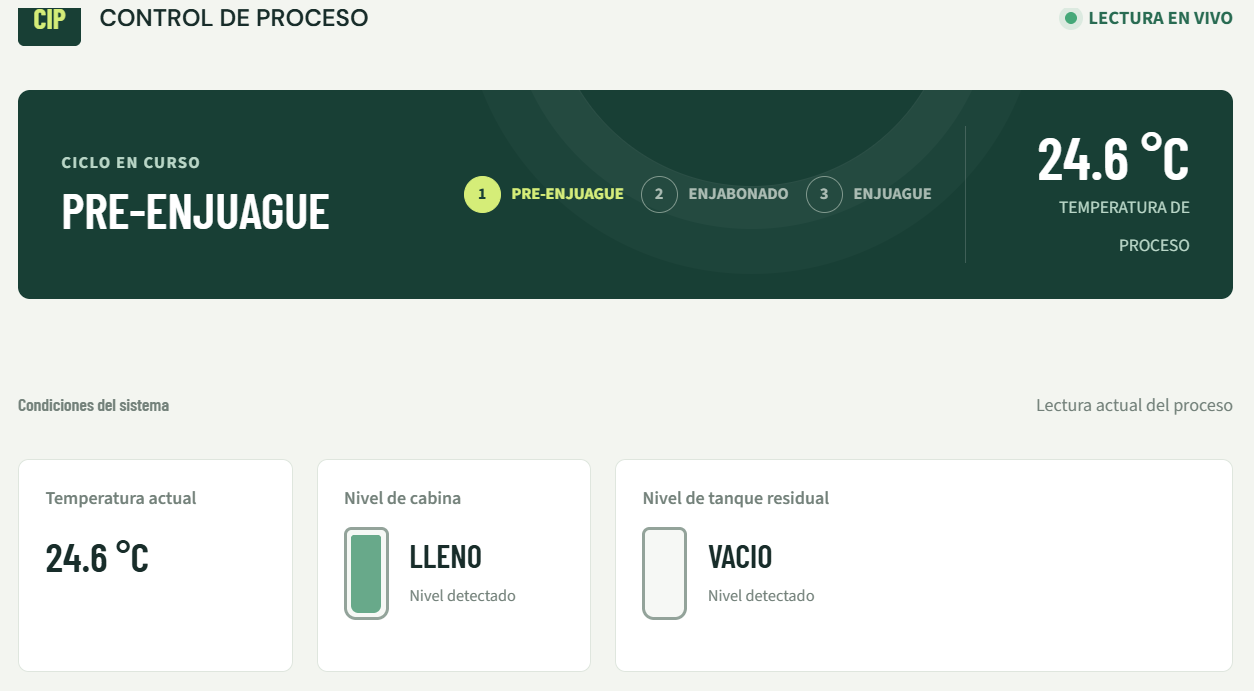
\includegraphics[width=0.62\textwidth]{interfaz_streamlit_proceso.png}\\[2mm]
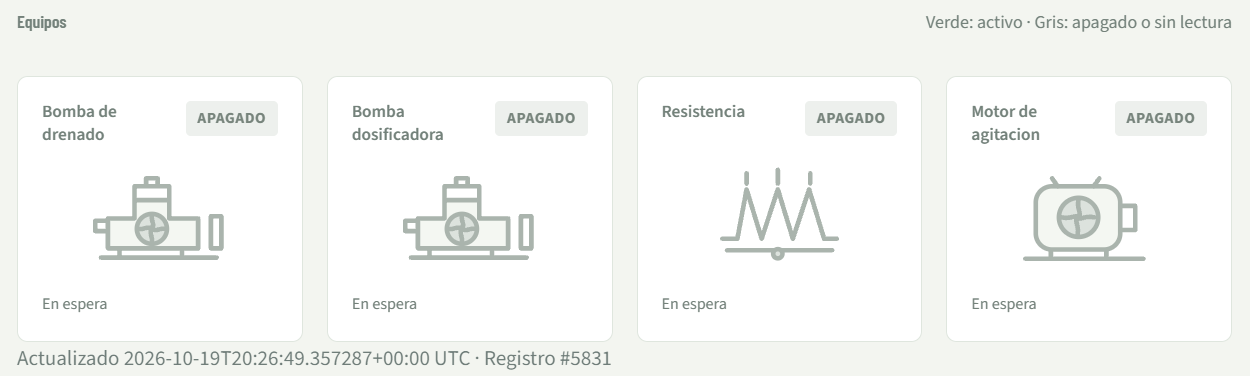
\includegraphics[width=0.62\textwidth]{interfaz_streamlit_equipos.png}
\caption{Interfaz web en Streamlit: fase del ciclo, temperatura, niveles y estado de los equipos (captura del 25 de noviembre de 2026, con la última lectura del 19 de octubre).}
\label{fig:interfaz_streamlit}
\end{figure}

\begin{figure}[H]
\centering
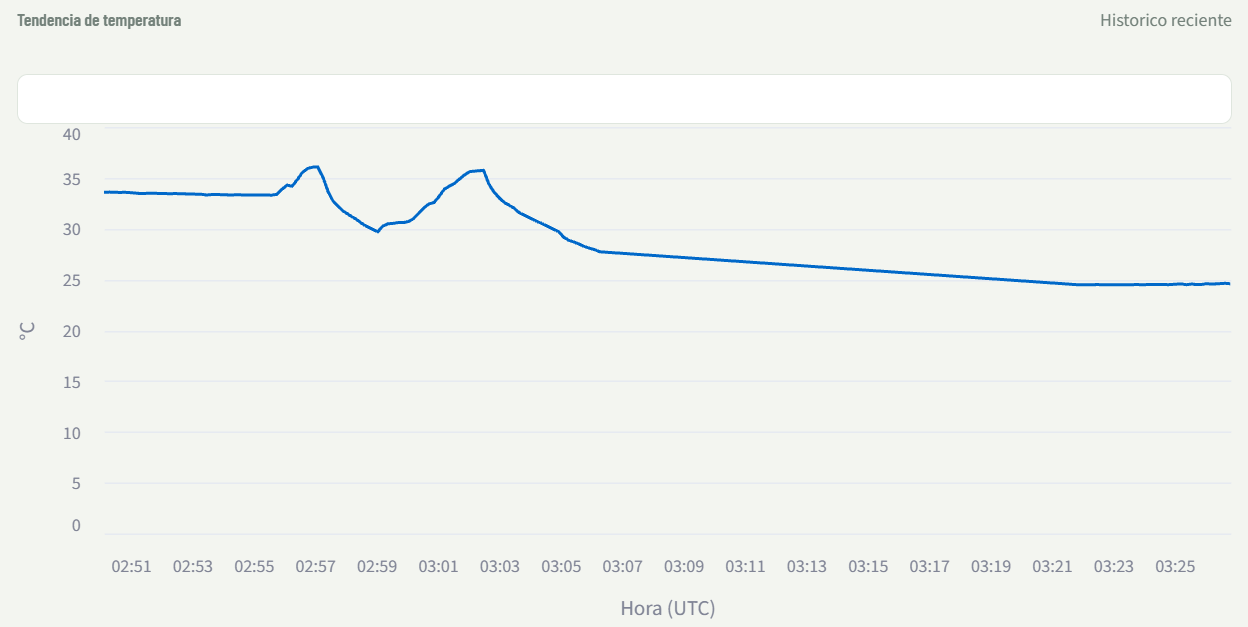
\includegraphics[width=0.78\textwidth]{interfaz_streamlit_tendencia.png}
\caption{Tendencia de temperatura en la interfaz web con las últimas 100 lecturas (19 de octubre de 2026). El eje indica UTC, pero muestra la hora local de Colombia en formato de 12 horas.}
\label{fig:interfaz_tendencia}
\end{figure}

\paragraph{Lecturas registradas.} La base de datos contiene 5831 lecturas, la última del 19 de octubre de 2026 a las 20:26:49 UTC (15:26:49, hora local), con 24,6\,°C, la fase de preenjuague y todos los equipos apagados. En las últimas 100 lecturas (Figura~\ref{fig:interfaz_tendencia}) se observan dos calentamientos que llegan a unos 36\,°C, valor que superaba el umbral de seguridad de 35\,°C vigente en esas pruebas, cada uno seguido de un descenso de la temperatura, y un tramo recto de unos 15\,min que sugiere que en ese intervalo no se recibieron lecturas. Descontado ese tramo, el intervalo medio estimado a partir de la gráfica es de unos 13\,s entre lecturas, por debajo de los 30\,s que exige el REQ-16. La verificación con el prototipo confirmó la actualización de las variables con un periodo de 30\,s o menos (VAL-10).

\paragraph{Estado de implementación.} Quedaron definidos la topología, los equipos, el protocolo principal y su alternativa, y la cadena de información; para la supervisión remota se adoptó la interfaz web en Streamlit, con FastAPI en el servidor. La aplicación móvil en Flutter que contempla el Anexo~\ref{anx:arquitectura_com} no forma parte de la versión adoptada. La cadena completa se verificó con el prototipo (VAL-10); queda pendiente la asignación definitiva de la dirección IP de la Raspberry Pi.

\paragraph{Limitaciones de la versión actual.} Al revisar el código frente al programa de la secuencia se identificaron los siguientes ajustes pendientes:
\begin{itemize}
\item La API solo acepta los valores 0, 1 y 2 para la fase. En el programa de la secuencia, \texttt{CICLO} aumenta al entrar a la etapa E7, de modo que durante el vaciado la interfaz ya mostraría la fase siguiente, y en el vaciado final (\texttt{CICLO} = 3) las lecturas no se guardarían. Las marcas \texttt{CICLO1}, \texttt{CICLO2} y \texttt{CICLO3} del Ladder v3 (Tabla~\ref{tab:db1_supervision}) sí conservan la fase correcta y pueden usarse en la supervisión.
\item La interfaz no distingue los estados de ciclo finalizado y de alarma que pide el REQ-17, y en reposo (\texttt{CICLO} = 0) muestra la fase de preenjuague. El programa del PLC ya entrega \texttt{Alarma\_Calent}, que puede enviarse a la API.
\item La interfaz avisa cuando la API no responde, pero no cuando la última lectura es antigua: en la Figura~\ref{fig:interfaz_streamlit} aparece \emph{lectura en vivo} aunque el último dato es de más de un mes antes.
\item El eje de tiempo de la gráfica indica UTC, pero muestra la hora local.
\item Cada lectura guarda solo la hora del servidor y no la hora del PLC, por lo que con estos datos no es posible calcular la latencia entre ambos.
\item El tanque de efluentes TK-103 no tiene sensor de nivel y Node-RED no lee ese dato, pero la interfaz muestra \texttt{VACIO} en ese campo, valor cuyo origen no se identificó.
\item En la función de Node-RED documentada en el repositorio, la variable de la bomba de impulsión se llama \texttt{Estado\_bomba\_drenado}, mientras que en la conexión S7 se llama \texttt{Estado\_bomba\_dreando}. Si la función instalada es la del repositorio, no encuentra esa variable y no envía la lectura, por lo que debe verificarse que ambos nombres coincidan.
\item La API trabaja con HTTP, sin cifrado ni autenticación, por lo que esta versión es solo para pruebas; antes de un uso permanente se deben incorporar HTTPS y autenticación.
\end{itemize}

\paragraph{Comportamiento ante pérdida de enlace.} La arquitectura está pensada para que una falla en la supervisión no afecte el proceso. Si se pierde la Raspberry Pi o el enlace WiFi, el PLC y la HMI siguen operando, y la API deja de recibir lecturas; el aviso de esta condición en la interfaz está pendiente. Lo mismo ocurre si se pierde internet: la función de Node-RED revisada no almacena lecturas, por lo que las de ese intervalo no quedan en el historial. Si se pierde la HMI, el PLC continúa su ciclo, y si el PLC se desconecta del switch, mantiene el control local del proceso. El caso de la HMI ya se verificó en el laboratorio 4 de Comunicaciones Industriales, con los mismos equipos: al desconectar la HMI durante 5\,s, el PLC siguió actualizando la temperatura y la HMI recuperó la visualización en 11,57\,s \cite{ruiz2026lab4}.

\paragraph{Pruebas de la cadena.} Para validar la cadena de comunicaciones se plantearon las siguientes pruebas; la del periodo de actualización se cumplió (VAL-10):
\begin{itemize}
\item Intercambio de dos variables: con un calibrador Fluke 726 se inyectan 4, 12 y 20\,mA en la entrada de temperatura y se verifica que Node-RED muestre el 0, el 50 y el 100\,\% del rango, como ya se verificó en el PLC y en la HMI en el laboratorio 4 (Sección~\ref{sec:montaje_pruebas}); además, se fuerza el nivel alto y se verifica el cambio de \texttt{true} a \texttt{false} de la señal de LSH-101, que es inversa, en la HMI y en Node-RED.
\item Periodo de actualización: medir, durante una prueba de 15\,min, el tiempo entre el PLC y la interfaz remota, para verificar el periodo máximo de 30\,s que exige el REQ-16.
\item Pérdida de enlace: desconectar la Raspberry Pi, la HMI y el enlace WiFi, uno a la vez, y verificar que el PLC mantiene el control local.
\item Evidencia: registrar capturas del flujo de Node-RED, de la interfaz remota y de la respuesta de la API.
\end{itemize}

El rango del transmisor TH200 (0 a 100\,\textdegree C) y el uso de la entrada analógica integrada de 0--10\,V con la resistencia de 500\,$\Omega$ ya se confirmaron en el laboratorio 4 \cite{ruiz2026lab4}.
